%% bare_jrnl.tex
%% V1.4
%% 2012/12/27
%% by Michael Shell
%% see http://www.michaelshell.org/
%% for current contact information.
%%
%% This is a skeleton file demonstrating the use of IEEEtran.cls
%% (requires IEEEtran.cls version 1.8 or later) with an IEEE journal paper.
%%
%% Support sites:
%% http://www.michaelshell.org/tex/ieeetran/
%% http://www.ctan.org/tex-archive/macros/latex/contrib/IEEEtran/
%% and
%% http://www.ieee.org/



% *** Authors should verify (and, if needed, correct) their LaTeX system  ***
% *** with the testflow diagnostic prior to trusting their LaTeX platform ***
% *** with production work. IEEE's font choices can trigger bugs that do  ***
% *** not appear when using other class files.                            ***
% The testflow support page is at:
% http://www.michaelshell.org/tex/testflow/


%%*************************************************************************

%% Legal Notice:
%% This code is offered as-is without any warranty either expressed or
%% implied; without even the implied warranty of MERCHANTABILITY or
%% FITNESS FOR A PARTICULAR PURPOSE! 
%% User assumes all risk.
%% In no event shall IEEE or any contributor to this code be liable for
%% any damages or losses, including, but not limited to, incidental,
%% consequential, or any other damages, resulting from the use or misuse
%% of any information contained here.
%%
%% All comments are the opinions of their respective authors and are not
%% necessarily endorsed by the IEEE.
%%
%% This work is distributed under the LaTeX Project Public License (LPPL)
%% ( http://www.latex-project.org/ ) version 1.3, and may be freely used,
%% distributed and modified. A copy of the LPPL, version 1.3, is included
%% in the base LaTeX documentation of all distributions of LaTeX released
%% 2003/12/01 or later.
%% Retain all contribution notices and credits.
%% ** Modified files should be clearly indicated as such, including  **
%% ** renaming them and changing author support contact information. **
%%
%% File list of work: IEEEtran.cls, IEEEtran_HOWTO.pdf, bare_adv.tex,
%%                    bare_conf.tex, bare_jrnl.tex, bare_jrnl_compsoc.tex,
%%                    bare_jrnl_transmag.tex
%%*************************************************************************

% Note that the a4paper option is mainly intended so that authors in
% countries using A4 can easily print to A4 and see how their papers will
% look in print - the typesetting of the document will not typically be
% affected with changes in paper size (but the bottom and side margins will).
% Use the testflow package mentioned above to verify correct handling of
% both paper sizes by the user's LaTeX system.
%
% Also note that the "draftcls" or "draftclsnofoot", not "draft", option
% should be used if it is desired that the figures are to be displayed in
% draft mode.
%
\documentclass[journal]{IEEEtran}
%
% If IEEEtran.cls has not been installed into the LaTeX system files,
% manually specify the path to it like:
% \documentclass[journal]{../sty/IEEEtran}

\bibliographystyle{IEEEtran}
\usepackage[none]{hyphenat}
\usepackage{graphicx}
\usepackage{float}
\usepackage{amsmath}
\usepackage{amsfonts}
\usepackage{amssymb}
\usepackage{dsfont}
\usepackage{textcomp}
\usepackage{url}

% Some very useful LaTeX packages include:
% (uncomment the ones you want to load)

% *** CITATION PACKAGES ***
%
% \usepackage{cite}
% cite.sty was written by Donald Arseneau
% V1.6 and later of IEEEtran pre-defines the format of the cite.sty package
% \cite{} output to follow that of IEEE. Loading the cite package will
% result in citation numbers being automatically sorted and properly
% "compressed/ranged". e.g., [1], [9], [2], [7], [5], [6] without using
% cite.sty will become [1], [2], [5]--[7], [9] using cite.sty. cite.sty's
% \cite will automatically add leading space, if needed. Use cite.sty's
% noadjust option (cite.sty V3.8 and later) if you want to turn this off
% such as if a citation ever needs to be enclosed in parenthesis.
% cite.sty is already installed on most LaTeX systems. Be sure and use
% version 4.0 (2003-05-27) and later if using hyperref.sty. cite.sty does
% not currently provide for hyperlinked citations.
% The latest version can be obtained at:
% http://www.ctan.org/tex-archive/macros/latex/contrib/cite/
% The documentation is contained in the cite.sty file itself.






% *** GRAPHICS RELATED PACKAGES ***
%
\ifCLASSINFOpdf
  % \usepackage[pdftex]{graphicx}
  % declare the path(s) where your graphic files are
  % \graphicspath{{../pdf/}{../jpeg/}}
  % and their extensions so you won't have to specify these with
  % every instance of \includegraphics
  % \DeclareGraphicsExtensions{.pdf,.jpeg,.png}
\else
  % or other class option (dvipsone, dvipdf, if not using dvips). graphicx
  % will default to the driver specified in the system graphics.cfg if no
  % driver is specified.
  % \usepackage[dvips]{graphicx}
  % declare the path(s) where your graphic files are
  % \graphicspath{{../eps/}}
  % and their extensions so you won't have to specify these with
  % every instance of \includegraphics
  % \DeclareGraphicsExtensions{.eps}
\fi

\begin{document}
%
% paper title
% can use linebreaks \\ within to get better formatting as desired
% Do not put math or special symbols in the title.
\title{Literature Study: A survey on using Identity Based Encryption for Online
Social Networks}
%
%
% author names and IEEE memberships
% note positions of commas and nonbreaking spaces ( ~ ) LaTeX will not break
% a structure at a ~ so this keeps an author's name from being broken across
% two lines.
% use \thanks{} to gain access to the first footnote area
% a separate \thanks must be used for each paragraph as LaTeX2e's \thanks
% was not built to handle multiple paragraphs
%

\author{Stijn Meul,
        ir. Filipe Beato,~\IEEEmembership{Supervisor}
        Prof. dr. ir. Bart Preneel,~\IEEEmembership{Promotor}
        Prof. dr. ir. Vincent Rijmen,~\IEEEmembership{Promotor}%
        }

% The paper headers
\markboth{}%
{}
% The only time the second header will appear is for the odd numbered pages
% after the title page when using the twoside option.
% 
% *** Note that you probably will NOT want to include the author's ***
% *** name in the headers of peer review papers.                   ***
% You can use \ifCLASSOPTIONpeerreview for conditional compilation here if
% you desire.

% make the title area
\maketitle

% As a general rule, do not put math, special symbols or citations
% in the abstract or keywords.
\begin{abstract}
In this paper the possibilities of realising user defined privacy in online
social networks (with Facebook in particular) based on identity-based
encryption and anonymous broadcast encryption are explored. The final goal is
to propose a practical useable implementation of increased user defined privacy
on Facebook.
\end{abstract}

% Note that keywords are not normally used for peerreview papers
% \begin{IEEEkeywords}
%IEEEtran, journal, \LaTeX, paper, template.
%\end{IEEEkeywords}






% For peer review papers, you can put extra information on the cover
% page as needed:
% \ifCLASSOPTIONpeerreview
% \begin{center} \bfseries EDICS Category: 3-BBND \end{center}
% \fi
%
% For peerreview papers, this IEEEtran command inserts a page break and
% creates the second title. It will be ignored for other modes.
\IEEEpeerreviewmaketitle



\section{Introduction} \label{sec:introduction}
\IEEEPARstart{O}{nline} Social Networks (\textit{OSNs}) are increasingly being
used to share sensitive data with a limited circle of online connections. Users
therefore have to count on the privacy infrastructure of the social network
itself. Social networks like Google Plus or Facebook realise these security
settings by defining groups of connections who are allowed to see certain
profile updates. At first sight the user seems protected from the general public
as it does not have access to these shielded updates. The OSN itself however
still has access to this data and gratefully uses it for comercial purposes like
targeted advertising or behavior analysis. All this data forms the basis of the
OSN's economical existence. As recent events have shown, this user data is not
only used for the sake of the OSN's financial survival but the data is leaked to
third parties and agencies like NSA as well. One can wonder if a company
non-transparently passes this data to any government agency for the argument of
security, what other purposes this data will be used for.\\
\\
Because the OSN has access to all users' data, it can be shared with external
parties. This takes the users' full control over their data completely out of
their hands. Additionally OSNs might offer API's to expose the users'
information to other services like external applications. Finally, OSNs
intentionally change security policies to maintain the balance between
usability and the commercial value of their databases thereby leaving their
users privacy behind.~\cite{BeatoScramble}\\
\\
One could argue that if one wants to stay anonymous, he should not use an OSN.
As the increasing popularity of OSNs has shown however, there is a market
demand for OSNs because of their wide range of useful applications. It would
therefore still be meaningful to make use of the infrastructure of a Social
Network without its inherent data leakage.\\
\\
The goal of this literature study is to research if an elegant architecture
exists that allows to keep using OSN infrastructure without having to rely on
the  willingness of OSNs to keep the user's data private. The study is done with
particularly Facebook in mind as this social network is amongst the most
popular ones in the world. In the end the user should be able to define his
own privacy instead of privacy policies being dictated by the social network.\\
\\
The structure of this paper is the following. First existing architectures
achieving similar privacy goals on social networks are discussed in
section~\ref{sec:existing-architectures}. Next an introduction to identity-based
encryption is given in section~\ref{sec:ibe} and which appealing properties make
IBE useful for increasing user defined privacy on Online Social Networks. In
section~\ref{sec:implementing-IBE-for-OSNs} different forms of broadcasting
schemes are considered for implementing IBE for Online Social Networks.
Finally, in section~\ref{sec:conclusion} a conclusion is given.


\section{Existing
Architectures~\cite{BeatoScramble}}\label{sec:existing-architectures}
Lots of fundamental work has been done on applications trying to enforce
access control rules on OSNs. A grasp of all available applications is
listed and analysed in the following section.

\paragraph{flyByNight} is a Facebook application that protects user data by
storing it in encrypted form in Facebook. It relies on Facebook servers for its
key management and is therefore not secure against active attacks by Facebook
itself.

\paragraph{NOYB (None Of Your Business)} replaces the details of user A with
those of random users B and C thereby making this process only reversible by
friends who are allowed to see the profile of user A. However this can not be
applied to user messages or status updates that are the most frequently used
features on Facebook.

\paragraph{FaceCloak} stores published Facebook data on its servers in encrypted
form and replaces the data on Facebook with random text fetched from Wikipedia.
This could be a useful mechanism to prevent OSNs from blocking security
aware users because they are scared to see their advertising revenues shrink.
However, this approach has the disadvantage that other users could take this
data to be genuine user content. Furthermore FaceCloaks architecture leads to an
inefficient key distribution system. 

\paragraph{Persona} is a scheme that can be used as a Firefox extension to let
users of an OSN determine their own privacy by supporting the ability to encrypt
messages to a group of earlier defined friends based on \textit{attribute-based
encryption (ABE)}\cite{SahaiFuzzyIBE}. The scheme supports lots of useful use
cases such as sending messages to all friends that are related to a certain
attribute or even encrypting messages to friends of friends. The major drawback
of this system however is that every new friend has to exchange a public key
before he is able to interact in the privacy preserving architecture
consequently requiring an infrastructure for broadcasting and storing public
keys. Furthermore, to support the encryption of messages to friends of friends,
user defined groups should be made available publicly thereby making the public
key distribution system even more complicated. Finally the proposed ABE
encryption scheme is 100 to 1000 times slower than a standard RSA operation.
\cite{BadenPersona} 

\paragraph{Scramble} is a Firefox extension that allows defining groups of
friends that are given access to certain social network updates. The tool uses
public key encryption based on OpenPGP \cite{rfc4880} to broadcast encrypted
messages on almost any platform. Furthermore Scramble provides the
implementation of a tiny link server such that OSN policies not allowing to post
encrypted data are bypassed. However, as indicated by usability studies
\cite{WhittenJohnny} OpenPGP has a higher usage threshold because an average
user does not manage to understand OpenPGP properly. Additionally Scramble has
to rely on the security decisions of the web of thrust. It therefore inherits
the upleasant property of OpenPGP that the user can not be sure that the used
PGP key actually belongs to the intended Facebook profile.\cite{BeatoScramble}\\
\\
The most unattractive property of all the above applications is that they have
to rely on a rather complex infrastructure. Persona has to support an extended
public key distribution system and Scramble relies on the leap-of-faith PGP web
of thrust. Would it not be pleasant to use an infrastructure that inherently
ensures that a Facebook update can only be read by the profiles the user
inteded to? Would it not be a desirable approach that Facebook would require
users to publish a public key on their Facebook profile such that communication
with external providers is limited to a minimum? As the most important part of
an OSNs' revenues lies in the data analysis of their users, the chances of
Facebook implementing a required public key option are rather low to
unexisting. To circumvent the requirement of such a public key attribute, it
would be user friendly if any unique public string could be used as a public
key. This is where identity based cryptography comes in.


\section{Identity Based Encryption}\label{sec:ibe}
Shamir proposed a concept of identity-based cryptography in
1984~\cite{DBLP:conf/crypto/Shamir84}. The basic idea behind identity-based
cryptography is that any string can be a valid public key for encryption or
signature verification thereby eliminating the need for digital certificates.
As a consequence identity-based cryptography reduces the system
complexity and the cost for establishing and managing the Public
Key Infrastructure (PKI). Identity-based cryptography proves to be particularly
elegant if the public key is related to an attribute that uniquely identifies
the identity of the user like an e-mail address, an IP address or a telephone
number~\cite{Baek04asurvey}.

\subsection{Working Principle~\cite{YoungbloodIntroduction}}
IBE relies on a thrusted third party called the \textit{Private Key Generator
(PKG)}. During the initialisation of the architecture the PKG generates a
public/private keypair called \textit{the master public key} $pk_{PKG}$ and
\textit{the master private key} $sk_{PKG}$. It is the master public key
$pk_{PKG}$ that is published publicly while the master private key $sk_{PKG}$
is kept secret.\\
\\
Once initialised, the secure exchange of packets takes place obeying the
following steps as shown in Figure~\ref{fig:ibe}:

\begin{enumerate}
 \item Alice uses Bob's identity $ID_{Bob}$ and the master public key $pk_{PKG}$
to encrypt a plaintext $M$ to a ciphertext $C$.
 \item Alice sends $C$ and some plaintext instructions $I$ over an insecure
channel to Bob.
 \item When Bob sees the ciphertext $C$, he uses the plaintext instructions $I$
to connect to the PKG. Bob authenticates with the PKG by sending sufficient
proof that $ID_{Bob}$ belongs to him.
 \item The PKG transmits Bob's private key $sk_{Bob}$ to him over a secure
channel.
 \item Bob recovers the plaintext message $M$ by decrypting it using his secret
key $sk_{Bob}$.
\end{enumerate}


\begin{figure}[H]
  \centering
  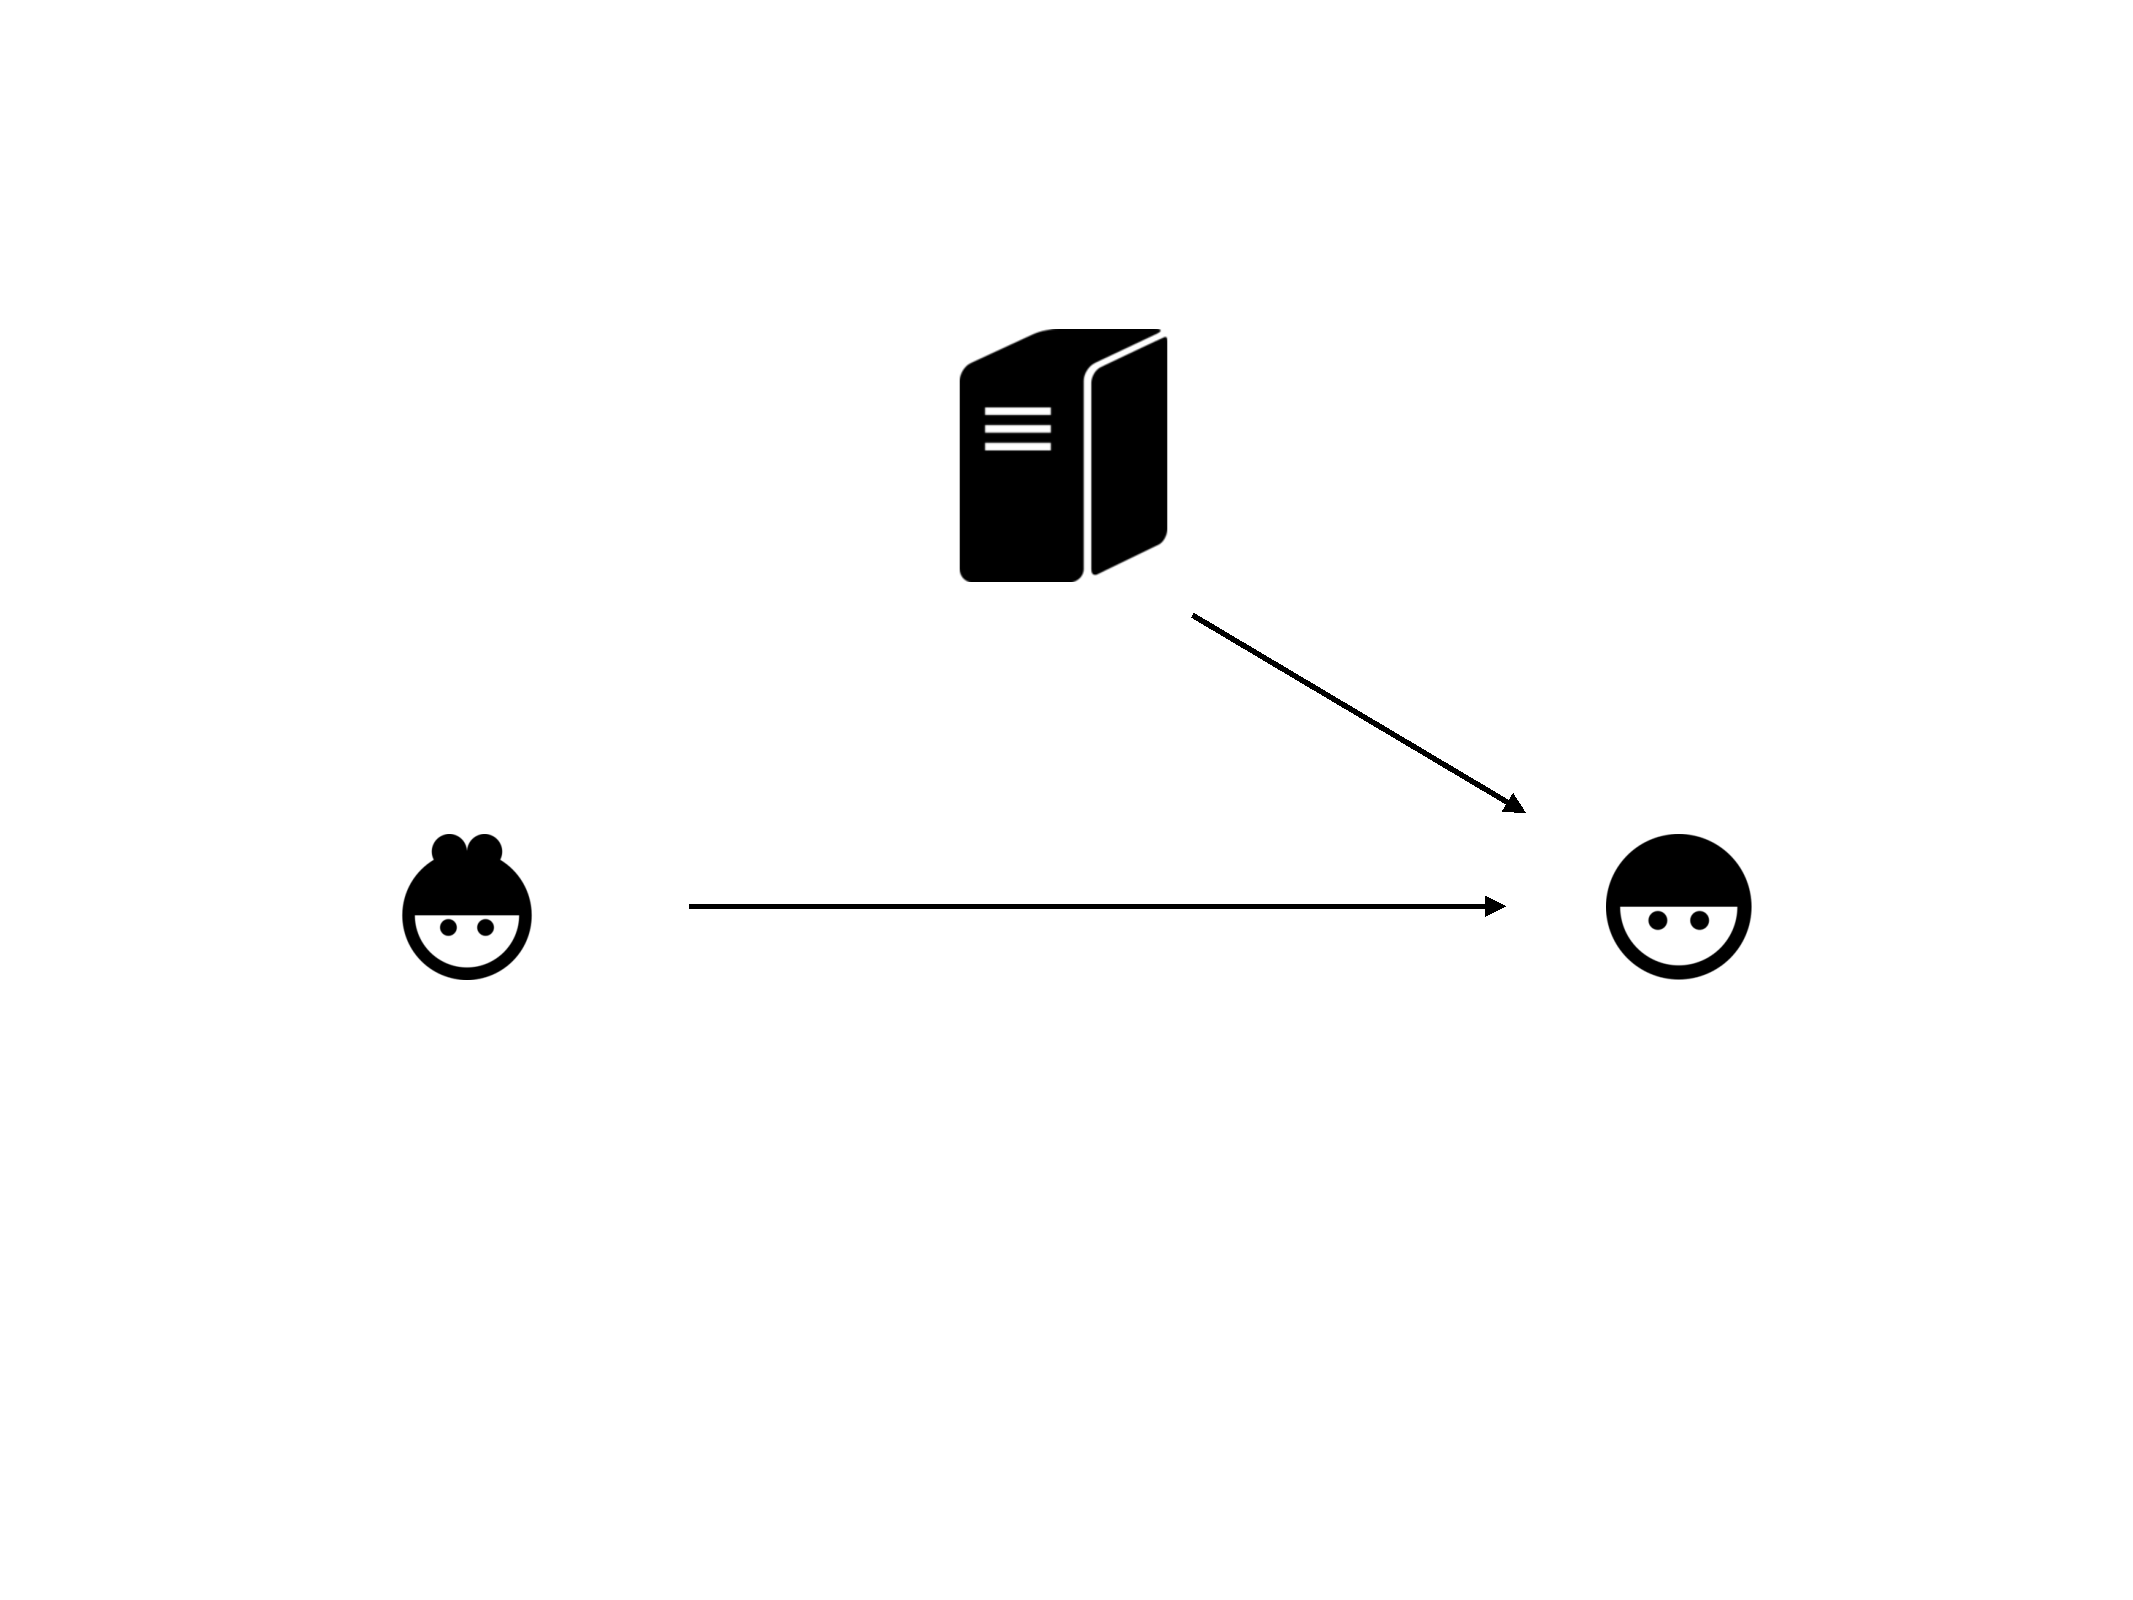
\includegraphics[width=3.5in,natwidth=772,natheight=326]{./img/ibe.jpg}
  \caption{Alice encrypting a message for Bob using Identity-Based Encryption}
  \label{fig:ibe}
\end{figure}

Please note that Alice does not require any prior actions from Bob to send him
an encrypted message. This is one of the major motivations to use IBE in a
practical setup. An attentive reader would remark however that this is realised
at the expense of key escrow. The PKG namely knows the secret key of Bob thereby
being able to decrypt every message that is sent to Bob. As the basic goal of
this study is to limit the omniscience of the social network this property is
very undesirable because the party to thrust has just shifted from the social
network to a third party PKG. Possible workarounds solving this issue are
discussed in Section~\ref{sec:possible-workarounds}.

\subsection{Pairings}\label{sec:pairings}
Although Shamir easily constructed an \textit{identity-based signature (IBS)}
scheme based on RSA in 1984, the use case of \textit{identity-based encryption
(IBE)} remained an open problem for many years. It was by the introduction of
\textit{bilinear maps} (also known as \textit{pairings}) that in 2001 Boneh and
Franklin\cite{BonehFranklinIBE} were able to implement the first secure and
truly practical IBE system~\cite{Baek04asurvey}.\\
\\
An IBE scheme can be built from any bilinear map $e : \mathds{G}_1 \times
\mathds{G}_1 \rightarrow \mathds{G}_2$ between two groups $\mathds{G}_1$ ,
$\mathds{G}_2$ as long as a variant of the Computational Diffie-Hellman problem
in $\mathds{G}_1$ is hard. Where $\mathds{G}_1$ and $\mathds{G}_2$ are two
groups of order $q$ for some large prime $q$. The bilinear map should satisfy
the following properties:

\begin{enumerate}
 \item Bilinear: A map $\hat{e}: \mathds{G}_1 \times \mathds{G}_1 \rightarrow
\mathds{G}_2$ is \textit{bilinear} if $\hat{e} \left(aP,bQ \right) = \hat{e}
\left( P,Q\right)^{ab}$ for all $P,Q \in \mathds{G}_1$
 \item Non degenerate: The map does not send all pairs in $e : \mathds{G}_1
\times \mathds{G}_1$ to the identity in $\mathds{G}_2$  such that if $P$ is a
generator of $\mathds{G}_1$ then $\hat{e}\left(P,P\right)$ is a generator of
$\mathds{G}_2$.
 \item Computable: There exists an efficient algorithm to compute
$\hat{e}\left(P,Q\right)$ for any $P,Q \in \mathds{G}_1$
\end{enumerate}

A bilinear map satisfying the above properties is called an \textit{admissible}
bilinear map. In other words it can be stated that an admissible bilinear map
is a function pairing elements from one cyclic group to another of the same
prime order, where the discrete log problem is hard in the first
group~\cite{YoungbloodIntroduction}. The group $\mathds{G}_1$ is a subgroup of
the additive group of points on an elliptic curve $E\textfractionsolidus
\mathds{F_{p}}$. The group $\mathds{G}_2$ is a subgroup of the multiplicative
group of points of a finite field $\mathds{F}_{p^{2}}^{*}$. Consequently
$\mathds{G}_1$ can be seen as an additive group and $\mathds{G}_2$ as a
multiplicative group.~\cite{BonehFranklinIBE}\\
\\
The security of IBE is based on the \textit{Bilinear Diffie-Hellman
Assumption (BDH assumption)}. This assumption states that given:
\begin{itemize}
 \item $\mathds{G}_1$ and $\mathds{G}_2$ groups of prime order $q$
 \item $\hat{e}: \mathds{G}_1 \times \mathds{G}_1 \rightarrow \mathds{G}_2$ an
admissible bilinear map
 \item $P$ a generator of $\mathds{G}_1$
 \item $\langle P, aP, bP, cP \rangle$ for some ungiven $a, b, c \in
\mathds{Z}_{q}^{*}$
\end{itemize}
it is computationally hard to calculate $W = \hat{e} \left( P , P \right)^{abc}$
although calculating $\langle P, aP, bP, cP \rangle$ for some given $a, b, c \in
\mathds{Z}_{q}^{*}$ and  $W = \hat{e} \left( P , P \right)^{abc}$ is fairly
easy once $a, b$ and $c$ are known~\cite{BonehFranklinIBE}. The admissible
pairing thus functions as a one-way function as it can be shown that solving the
BDH assumption is reducible to solving the discrete-log problem for these
bilinear maps~\cite{YoungbloodIntroduction}.\\
\\
Both modified Weil and Tate pairings suffice the required properties for
admissable bilinear maps and are used in practice. Tate pairings however have
the advantage of being computationally more efficient then Weil
pairings~\cite{YacovBilinear}.\\
\\
Please further note that:
\begin{equation} \label{eq:sym}
 \hat{e} \left( aX, bY\right) = \hat{e} \left( X, Y\right)^{ab} = \hat{e} \left(
bX, aY\right)
\end{equation}
where $aX$ represents a multiplication of a point on an elliptic curve by
integers. Although the multiplication operation $aX$ is easy, finding $a$ given
$aX$ will be computationally infeasible~\cite{YoungbloodIntroduction}.

\subsection{A Concrete IBE Scheme}
Pairings as dicussed in Section~\ref{sec:pairings} allow to implement a
concrete IBE scheme based on the following 4 steps:

\begin{enumerate}
 \item \textit{Setup}: the PKG picks an elliptic curve, a  random secret $s$ and
a point $P$ on the curve. $P$ and $sP$ are made public such that $pk_{PKG}$ =
$\langle P, sP\rangle$ in Figure~\ref{fig:ibe}.
 \item \textit{Encryption}: As Alice knows $pk_{PKG}$ and $ID_{Bob}$, she can
pick a random $r$ and calculate a key $k$ to encrypt her plaintext message $M$
by $k = \hat{e} \left( r ID_{Bob}, pk_{PKG}\right)= \hat{e} \left( r ID_{Bob},
sP \right)$. Alice then sends $\langle Encrypt_{k}\left( M \right), rP \rangle$
to Bob.
 \item \textit{Extract:} If Bob has never received a message before, he still
needs to receive its private key from the PKG. Bob authenticates with the PKG
after which the PKG calculates $sk_{Bob} = s ID_{Bob}$ and returns this to Bob
over a secure channel.
 \item \textit{Decryption:} Bob can now calculate the key $k$ to decrypt
$\langle Encrypt_{k}\left( M \right)$ by $k = \hat{e} \left( s ID_{Bob}, rP
\right)$.
\end{enumerate}
Note that the key $k$ calculated by Bob and the key $k$ calculated by Alice is
the same because of the property illustrated in Formula~\ref{eq:sym}.
Furthermore Bob and the PKG are the only ones able to decrypt $Encrypt_{k}\left(
M \right)$ as nobody else knows $s ID_{Bob}$.

\subsection{Security Definitions}
In all research concerning IBE, whether it is pure pairing based IBE or more
complex broadcasting schemes, some definitions about an algorithm's level of
security are always considered. Although most of these security definitions
change depending on the considered algorithm, there are some general concepts
that are similar.\\
\\
The security level of an algorihm is mostly defined based on an attackers game.
The more actions an attacker is allowed to perform in this game without gaining
any advantage in trying to decrypt messages, the safer the algorithm. Although
this is very roughly stated, it is a concept that is encountered frequently in
literature.\\
\\
In IBE there are mainly two accepted definitions of security:
\begin{enumerate}
 \item \textit{Full security} which means the attacker can choose adaptively the
identity he wants to attack after having seen the parameters of the algorithm.
 \item \textit{Selective-ID security} which means that the attacker must choose
the identity he wants to attack at the beginning, before seeing the paramters.
\end{enumerate}
As the attacker is more restricted in its actions in Selective-ID security it
is considered less secure.~\cite{DelerableeIBBE}\\
\\
Another notion that frequently appears in literature covering IBE is the concept
of \textit{random oracles}. A random oracle is a black box that responds to
every unique query with a (truly) random response chosen uniformly from its
output domain, except that for any specific query, it responds the same way
every time it receives that query. Very often, random oracles are used in
security proofs to model true randomness. In reality these oracles are often
implemented by hash functions. Therefore proving security based on true random
oracles is easier than proving the actual implementation of an algorithm to be
secure. However, an application that does not require random oracle heuristics
is considered to be safer.~\cite{WikiOracle}

\subsection{Advantages of IBE}
As already mentioned in Section~\ref{sec:ibe} one of the most attractive
properties of IBE is the recipient that does not have to have taken any action
before being able to start receiving messages. Certainly in an OSN this would
be a compelling feature as the user does not have to upload its public key to a
key ring neither to a public server. For the public key, any string
that uniquely identifies a user can be used. If a string is chosen that is
inherently part of the OSN's architecture, the user does not have to perform
actions that are incromprehensible to him. The ideal case is that once the
user has signed up for the service of the OSN, he is ready to receive encrypted
messages without taking any additional decisions concerning key lengths or
algorithmic properties.\\
\\
Moreover, an IBE architecture reduces the complexity of the system as there is
no further need for public key certificates. The user only has to receive his
secret key once from the PKG over a secure channel. After he knows his private
key, the user theoretically never has to contact the PKG again unless he loses
his private key. The contrast in complexity with a CA hierarchy and security
certificates being issued periodically is immense.\\
\\
Finally, IBE has less restrictions on scaling because PKGs can be distributed
independently and geographically without the need to synchronise data. This
property enables quick and easy key management all over the
world.~\cite{VoltageIBE}

\subsection{Disadvantages of IBE}\label{sec:possible-workarounds}
One of the major drawbacks of IBE is its inherent key escrow property. If one
does not want to trust his data to a provider of an OSN, he probably does
not want any other unintended third party to have access to this data either. A
possible countermeasure for the above key escrow problem would be to use
Shamir's secret sharing technique to distribute the PKG's master secret key
$sk_{PKG}$ over a number of different PKGs~\cite{BonehFranklinIBE}. But as this
method requires users to authenticate themselves to multiple PKGs, this
workaround increases the total communication and computational cost of the
system~\cite{Baek04asurvey}.\\
\\
Another disadvantage of IBE is that \textit{Certificate Revocation Lists (CRLs)}
are no longer supported as there are no security certificates to revoke. At
first sight this seems a good thing as supporting CRLs is cumbersome and puts
heavy demands on the individual users of a PKI. However, this also implies that
public keys can not be revoked in case their coresponding private keys are
compromised. Such a scenario would imply that the user could no longer make use
of certain strings that are immediately linked to his identity. To get around
this issue a validity timestamp could be concatenated to the ID component
thereby limiting the period during which a public key would be valid. By doing
so, restrictions would be placed on the duration the compromised
secret key. Remark that such a workaround would imply a
higher computational and communication cost as well because all users have to
reconnect over the secure channel to the PKG asking for a new secret key every
time their timestamp expires~\cite{YoungbloodIntroduction}.

\section{Implementing IBE for Online Social
Networks}\label{sec:implementing-IBE-for-OSNs}
As Scrambe~\cite{BeatoScramble} already has a user friendly interface that
supports all required actions to implement encryption on Online Social Networks,
it would be useful to alter the existing Scramble code that it can implement
IBE as well. The most important trigger to modify the existing Scamble code is
because Scramble is open source, lightweight and developed at KU Leuven.
Certainly the latter argument eases the process of altering the existing code
and therefore is an asset.

\subsection{User Public Key}
The most important design decision is which profile attribute to use as a public
key string of the user. The desired properties for such a user public key
(denoted $ID_{Bob}$ in Figure~\ref{fig:ibe}) are the following:
\begin{enumerate}
 \item The public key should uniquely identify the user
 \item The public key should be mandatory for every user of the social network
 \item The public key should not change frequently over time
 \item The public key should be an inherent part of the infrastructure of the
social network thereby meaning that the previous three properties are already
ensured by the provider of the social network.
\end{enumerate}
Please note that the decision of which string to use as a public key, is
highly dependent on the targeted social network. Every OSN will namely have
other profile attributes satisfying the earlier mentioned properties. Scramble
would therefore become platform dependent. However, this is an offer the writers
of this paper are willing to make for the sake of an increased ease of use.\\
\\
As already mentioned in Section~\ref{sec:introduction} the focus of this paper
will be on Facebook although other OSNs could make use of the concepts
mentioned in this paper. In Facebook there is a very obvious and readable
string satisfying the earlier mentioned properties namely the Facebook
username.\\
\\
A Facebook username is an unique identifier that serves as an URL of
someone's profile. For example \texttt{http://www.facebook.com/user.name}
refers to the Facebook profile of the user with Facebook username
\texttt{user.name}.\\
\\
Using the username as an identifier ensures that all the above properties are
satisfied as an URL can only refer to one page. Because every Facebook page is
reachable using an URL, every user has such a username. Furthermore, the public
key does not change frequently over time as Facebook limits changing this string
only once~\cite{FacebookUsername}. Finally, Facebook has the responsibility to
check all these properties as URL collisions would occur if they did not take
care of this.\\
\\
Additional pleasant properties are that user names are:
\begin{enumerate}
 \item mostly closely related to the identity of the user. 
 \item mostly readable as users choose them to make their profile easier to
reach using an URL. This property also makes them easier to remember.
\end{enumerate}


\subsection{IBE Broadcasting}
\textit{Broadcast Encryption (BE)} techniques ensure confidentiality when
sending a message to an arbitrary subset drawn from a universe of users. The
universe of users is usually called $U$ and the set of targeted users is
denoted with $S$ such that $S \subseteq U$. The concept of Broadcast Encryption
was originally introduced by Fiat and Naor~\cite{FiatBE} in
1993~\cite{LibertANOBE}. A BE scheme is said to be \textit{fully collusion
resistant} when, even if all users that are not in $S$ collude, they can by no
means infer information about the broadcast message.~\cite{DelerableeIBBE} \\
\\
If one wants to encrypt the same message $M$ for a large set of identities, one
can simply encrypt $M$ seperateley for each individual identity and then
transmit these encrypted messages separately. If the cardinality of the set of
targeted identities is $|S|$, then one has to perform $|S|$ independent
encryptions. Of course such a solution would be too expensive in terms of
bandwidth requirement as well as pairing computation. Baek, Safavi-Naini and
Susilo in~\cite{BaekIBEandBE} addressed this problem for the first time in
literature. They call their protocol \textit{Multi Receiver Identity-Based
Encryption (MR-IBE)} and base it on the Boneh-Franklin IBE using bilinear
pairings. In their paper, Baek et al. prove MR-IBE to be secure in the
selective-ID model using the random oracle heuristic. Independent of this work,
Barbosa and Farshim~\cite{BarbosaIBEKEM} proposed an identity-based key
encapsulation scheme for multiple parties which is an extension of \textit{mKEM}
as proposed by Smart~\cite{SmartMKEM} to the identity-based
setting. An mKEM is a Key Encapsulation Mechanism which takes multiple public
keys as input. An encrypted message under mKEM consists of an encapsulated
session key $K$ and a symmetric encryption of the plaintext message $M$ under
$K$. In this way only the encapsulation of the key uses computation intensive
public key encryption~\cite{SmartMKEM}. Barbosa and Farshim prove their
algorithm to be secure under random oracle assumptions. Later
constructions based on the Boneh-Boyen (H)IBE~\cite{ChatterjeeHIBE} even show
security without using the random oracle heurstic.
~\cite{ChatterjeeShortenedCiphertext}\\
\\
The first proposals for these indentity-based broadcasting schemes had some
undesirable properties like public key lengths being determined by the total
number of possible users $|U|$. Lots of research optimising
identity-based broadcasting schemes has been done since then to improve on the
efficiency and usability of the original proposals. Delerabl\'ee introduces an
Identity Based Broadcast Encryption scheme with constant sized ciphertext and
private keys and a public key that is linear in the maximal number of
receivers $|S|$. This is an improvement on earlier defined
architectures as the maximum number of users is no longer fixed by the public
key length. These improvements are realised by using broadcast KEM-DEM
techniques. However, it is required in this architecture that the targeted set
of receivers $S$ is broadcasted to all users as well thereby leaking a lot of
information.~\cite{DelerableeIBBE}

\subsection{Anonymous Broadcast Encryption}
It is maybe useful to take one step back and think about the consequences of
all intended receivers being published in plain text together with the encrypted
message on a Social Network. If for example Bob's girlfriend celebrates her
birthday in a few weeks and he spreads an encrypted message to all her friends
without including her as a recipient, she will probably know Bob is up to
something. This is just one example of possible many that illustrates the
negative impact on security broadcasting of $S$ can have in real life
situations. Depending on the context, information can be deduced about a
status update without decrypting the update to plain text.\\
\\
Broadcast encryption schemes that do not leak information about the intended
recipients are called \textit{Anonymous Broadcasting Encryption (ANOBE)}
schemes.~\cite{LibertANOBE} As these systems do not profit from $S$ being known
to every user upfront they are less efficient than non-anonymous BE
schemes. Thus there clearly is a tradeoff between secrecy and efficiency in
ID-based Broadcasting architectures although this tradeoff can be
partially cancelled by letting the sender precompute certain
parameters~\cite{FanANOMIBE}.\\
\\
Fan et al.~\cite{FanANOMIBE} are the first to consider the anonymity of the
receivers in an ID-based broadcasting encryption architecture. They propose a
protocol based on Lagrange interpolating polynomials such that anonymity is
preserved for every receiver against any other receiver. All users of the
system $U$ can analyse whether they are an intended receiver or not while only
the sender knows who the other receivers in $S$ are. Wang et al. show
in~\cite{WangCryptanalysis} that the original architecture as proposed
in~\cite{FanANOMIBE} does not provide the level of anonymity as originally
intended because everyone is able to deduce the set of authorised identities.
In~\cite{WangCryptanalysis} protocol changes fixing these weaknesses are
suggested and prove is given that the improved scheme satisfies the
confidentiality and receiver anonymity under random oracle assumptions. Also
Chien~\cite{ChienImproved} proposes similar improvements on the original
architecture by Fan et al.~\cite{FanANOMIBE} Zhang et al.~\cite{ZhangComment}
point out that the scheme of Wang et al. is not safe either as all authorised
users in $S$ can deduce which other users are in $S$. In their paper a
solution is presented to this issue as well as some computational improvements
compared to Wang et al.'s scheme.\\
\\
Note however that although receivers being secret to unintended other users is
desirable, it might be useful on a social network that the members of the set
$S$ know each other. Suppose for example that Alice posts a Facebook update on
her profile page intended to Bob and Dylan. This means that $Bob, Dylan \in S$.
As a reaction to Alice's Facebook update, Bob wants to write a reply to start a
discussion. However, as Bob does not know which other users are allowed to see
Alice's update, he can now only encrypt his reply to Alice thereby preventing
Dylan from joining the discussion. However, this discussion could have been
useful to Dylan as well because otherwise Alice would not have included Dylan
as a recipient in $S$ in the first place. A workaround for this issue could be
to concatenate $S$ to the plaintext message $M$ such that $M || S$ is encrypted
instead of $M$. Currently possible algorithms taking a computational advantage
of the broadcasting of $S$ in an encrypted form, are not known to the writers
of this paper.

\section{Conclusion}
Identity-Based Encryption (IBE) seems to have desirable properties for
implementations increasing user defined privacy in OSNs. Mainly the minimal
additional architectural support and the increased ease of use, are major
motivations to implement IBE in Online Social Network (OSN) environments. Some
disadvantages like a lack of key revocation and implicit key escrow are
unpleasant but can be solved at the expense of increasing the complete system's
complexity.\\
\\
Broadcast Encryption (BE) techniques can be used to optimise the required
bandwidth and computational cost. Anonymous Broadcast Encryption (ANOBE)
techniques even protect the identity of the authorised receivers.
Anonymous Identity-Based Broadcast Encryption combines all desirable properties
to a prefered architecture for IBE in OSNs although this still is a fast
changing research domain.\\
\\
For a practical implementation of IBE on an OSN, Scramble could be rewritten
that it supports Anonymous Identity-Based Broadcast Encryption on Facebook by
using Facebook usernames as public keys. The key escrow property of IBE could
be circumvented using a threshold secret sharing setup. The inability to revoke
public keys could be compensated by appending a validity period to each public
key in a standardised fashion such that the architecture implicitly knows when
to issue new private/public key pairs.\cite{GentryRandomOracles} t \cite{FazioOutsiderANOBE} s \cite{BarthBonehWaters} e \cite{BoldyrevaRevocation} f \cite{GentryRandomOracles}
% if have a single appendix:
%\appendix[Proof of the Zonklar Equations]
% or
%\appendix  % for no appendix heading
% do not use \section anymore after \appendix, only \section*
% is possibly needed

% use appendices with more than one appendix
% then use \section to start each appendix
% you must declare a \section before using any
% \subsection or using \label (\appendices by itself
% starts a section numbered zero.)
%



\appendices


% Can use something like this to put references on a page
% by themselves when using endfloat and the captionsoff option.
\ifCLASSOPTIONcaptionsoff
  \newpage
\fi


% trigger a \newpage just before the given reference
% number - used to balance the columns on the last page
% adjust value as needed - may need to be readjusted if
% the document is modified later
%\IEEEtriggeratref{8}
% The "triggered" command can be changed if desired:
%\IEEEtriggercmd{\enlargethispage{-5in}}

% references section

% can use a bibliography generated by BibTeX as a .bbl file
% BibTeX documentation can be easily obtained at:
% http://www.ctan.org/tex-archive/biblio/bibtex/contrib/doc/
% The IEEEtran BibTeX style support page is at:
% http://www.michaelshell.org/tex/ieeetran/bibtex/
% \bibliographystyle{IEEEtran}
% argument is your BibTeX string definitions and bibliography database(s)
%\bibliography{IEEEabrv,../bib/paper}
%
% <OR> manually copy in the resultant .bbl filer
% set second argument of \begin to the number of references
% (used to reserve space for the reference number labels box)
\bibliography{references}




%\begin{thebibliography}{1}
%\bibitem{IEEEhowto:kopka}
%H.~Kopka and P.~W. Daly, \emph{A Guide to \LaTeX}, 3rd~ed.\hskip 1em plus
%  0.5em minus 0.4em\relax Harlow, England: Addison-Wesley, 1999.
%\bibitem{}

%\end{thebibliography}



% that's all folks
\end{document}
